\documentclass[final]{beamer}
%\usetheme{CASE_ASICS}
\usetheme{CASE_WirelessCommunications}


%%%%%%%%%%%%%%%%%%%%%%%%%%%%%%%%%%%%%%%%%%%%%%%%%%%%%%%%%%%%%%%%%%%%%%%%%%%%%%%
% BEGIN packages includes
\usepackage{etex}

\usepackage[orientation=portrait,size=a1,scale=1.4,debug]{beamerposter}
\usepackage[absolute,overlay]{textpos}
\setlength{\TPHorizModule}{1cm}
\setlength{\TPVertModule}{2.35cm}
\usepackage{ragged2e}
\usepackage{grffile}
\usepackage{mathtools}        % loads »amsmath«
\usepackage{amsmath,amsthm,amssymb,latexsym}
\DeclarePairedDelimiter\ceil{\lceil}{\rceil}
\DeclarePairedDelimiter\floor{\lfloor}{\rfloor}
\usepackage{array,booktabs,tabularx}

\usepackage{pgf}
\usepackage{tikz}
%\usepackage{gnuplot-lua-tikz}

\usepackage{wrapfig}

\usepackage{multirow}
% END packages includes
%%%%%%%%%%%%%%%%%%%%%%%%%%%%%%%%%%%%%%%%%%%%%%%%%%%%%%%%%%%%%%%%%%%%%%%%%%%%%%%


%%%%%%%%%%%%%%%%%%%%%%%%%%%%%%%%%%%%%%%%%%%%%%%%%%%%%%%%%%%%%%%%%%%%%%%%%%%%%%%
% BEGIN title, authors and references
\title{Low size FFT core for OFDM communications}
\author{
   Andres~D.~Cassagnes{\small*},~Federico~G.~Zacchigna{\small*},~Octavio~Alpago{\small*}~and~Ariel~Lutenberg{\small* \small**}\\
   {\small *Laboratorio~de~Sistemas~Embebidos~(FIUBA)~\small **CONICET-GICSAFe}}


\newcommand{\contactauthor}{Laboratorio de Sistemas Embebidos\\
                           Facultad de Ingeniería - UBA\\
                           Paseo Col\'on 850, CABA\\
                           E-mail: andres.cass@gmail.com\\
                           ~}

\newcommand{\Refauthor}{
%   [1] Dong Wentao; Li Wenfeng; Zhang Fan, ``Consensus algorithm for energy consumption of wireless sensor networks,'' Systems, Man, and Cybernetics (SMC), 2011 IEEE International Conference on , vol., no., pp.2620,2625, 9-12 Oct. 2011
%   doi: 10.1109/ICSMC.2011.6083992

%   [2] Chunhua Sun; Wei Zhang; Ben, K., ``Cluster-Based Cooperative Spectrum Sensing in Cognitive Radio Systems,'' Communications, 2007. ICC '07. IEEE International Conference on , vol., no., pp.2511,2515, 24-28 June 2007
%   doi: 10.1109/ICC.2007.415

%   [3] Ian F. Akyildiz, Brandon F. Lo, and Ravikumar Balakrishnan. 2011. ``Cooperative spectrum sensing in cognitive radio networks: A survey.'' Phys. Commun. 4, 1 (March 2011), 40-62.
%   DOI=10.1016/j.phycom.2010.12.003 http://dx.doi.org/10.1016/j.phycom.2010.12.003

%  [1] Rago, Constantino; Willett, P.; Bar-Shalom, Y., ``Censoring sensors: a low-communication-rate scheme for distributed detection,'' Aerospace and Electronic Systems, IEEE Transactions on, vol.32, no.2, pp.554,568, April 1996
%   doi: 10.1109/7.489500
  [1] Cassagnes, A., Lutenberg, A., Giordano Zacchigna, F. (2016) ``Implementacion y analisis de algoritmos de calculo de Transformada Rapida de Fourier para su aplicacian en sistemas OFDM''
  http://laboratorios.fi.uba.ar/lse/tesis/LSE-FIUBA-Tesis-Grado-Andres-Cassagnes-2016.pdf
                                    
  [2] Prasad, R. (2004), Orthogonal Frequency-Division Multiplexing. In \textit{OFDM for Wireless Communications Systems} (p.p. 11-15), UK: Artech House.
  
  [3] Melo, R., Salom\'on, F., Valinoti, B., (2016) ``IP core FFT configurable en Runtime''
%   doi: 10.1109/SASE-CASE.2014.6914462

%   [6] Pereira, S.S.; Pages-Zamora, A., ``Consensus in Correlated Random Wireless Sensor Networks,'' Signal Processing, IEEE Transactions on , vol.59, no.12, pp.6279,6284, Dec. 2011
%   doi: 10.1109/TSP.2011.2166552
}
% END title, authors and references
%%%%%%%%%%%%%%%%%%%%%%%%%%%%%%%%%%%%%%%%%%%%%%%%%%%%%%%%%%%%%%%%%%%%%%%%%%%%%%%


%%%%%%%%%%%%%%%%%%%%%%%%%%%%%%%%%%%%%%%%%%%%%%%%%%%%%%%%%%%%%%%%%%%%%%%%%%%%%%%
\begin{document}
\begin{frame}{}
%%%%%%%%%%%%%%%%%%%%%%%%%%%%%%%%%%%%%%%%%%%%%%%%%%%%%%%%%%%%%%%%%%%%%%%%%%%%%%%
\begin{columns}




%%%%%%%%%%%%%%%%%%%%%%%%%%%%%%%%%%%%%%%%%%%%%%%%%%%%%%%%%%%%%%%%%%%%%%%%%%%%%%%
%%%%%%%%%%%%%%%%%%%%%%%%%%%%%%%%%%%%%%%%%%%%%%%%%%%%%%%%%%%%%%%%%%%%%%%%%%%%%%%
% BEGIN first column
% -----------------------------------------------------------------------------
% Set up a column
\begin{column}{.5\textwidth}
   \begin{beamercolorbox}[center,wd=0.9\textwidth]{postercolumn}
      \begin{minipage}[T]{.99\textwidth}
      \parbox[t][105cm]{\textwidth}{

%%%%%%%%%%%%%%%%%%%%%%%%%%%%%%%%%%%%%%%%%%%%%%%%%%%%%%%%%%%%%%%%%%%%%%%%%%%%%%%
% BEGIN Introduction and objectives
        \begin{block}{Introduction and objectives}
          \justify
          One of the most used modulation schemes in communication systems that fulfills the current data bandwith demand is the 
          Orthogonal Frequency Division Multiplexing (OFDM), which transmits the data  over multiple orthogonal carriers.
          The main advantage of the OFDM over other multi-carrier modulations is the carrier orthogonality, which permits to overlap 
          the spectrum of the carriers without getting any inter-carrier interference.
          
          The OFDM modulation scheme can be expressed as:
			%
			\begin{equation}
			s_{k}(t-kT) =
			%	\begin{cases}
				\sum\limits_{i=-N/2}^{N/2-1} x_{i,k} e^{j2\pi
				\left(\frac{i}{T}\right)(t-kT)}
			%	\end{cases}
			\label{eq:OFDM_symbol_low}
			\end{equation}
			where $x_{i,k}$ is the $i$th data symbol associated to the $k$th sub-carrier, and $T$ is the symbol period.
			It is easy to recognize in (\ref{eq:OFDM_symbol_low}) an Inverse Discrete Fourier Transform. 
			Assuming that $x_{i,k}$ is constant along the symbol period $T$ it is possible to use an Inverse Discrete Fourier Transform\slash Discrete Fourier Transform
			(IDFT\slash DFT) blocks to modulate\slash demodulate the OFDM signal, which might be computed by using the efficient Fast Fourier Transform (FFT) algorithm, 
			which reduces the complexity of the algorithm from $\mathcal{O}(n^2)$ to $\mathcal{O}(n \, log n)$
			
			The objective of this work is to obtain an FFT core, small enough to be included in a complete OFDM transceiver without consuming 
			too much resources, but efficient and accurate enough to be useful in an ISDB-T television system.
			
			The main requirements for the implementation can be summarized in:
%
			\begin{itemize}
			  \item Run-time configurable FFT length, including at least 2K, 4K and 8K samples \cite{ISDB}.
			  \item $8,126,984$ sampling frequency guaranteed \cite{ISDB}.
			  \item Continuous input and output (not burst mode).
			  \item Fixed point arithmethics.
			  \item Run-time configurable and step-selectible scaling, with rounding and clipping options.
			  \item Lower space consuption than other implementations, taking as references Xilinx IP and an open FFT for ISDB-T OFDM implementation.
			\end{itemize}
			
        \end{block}
% END Introduction and objectives
%%%%%%%%%%%%%%%%%%%%%%%%%%%%%%%%%%%%%%%%%%%%%%%%%%%%%%%%%%%%%%%%%%%%%%%%%%%%%%%


%%%%%%%%%%%%%%%%%%%%%%%%%%%%%%%%%%%%%%%%%%%%%%%%%%%%%%%%%%%%%%%%%%%%%%%%%%%%%%%
% BEGIN MESA algorithm
	    \begin{block}{Implementation}
	    	\justify
	    	
			Radix-r algorithms reduces the calculation of one n-point FFT to the calculation of $\nu$ smaller r-point sub-FFTs where $N = r^\nu$. This leads to the posibility of
			reuse the same modules for all the r-point FFT computation.\\
			
			As the main objective is to achieve a low size core, an iterative version is chosen for implementation because it uses only one r-point FFT core for all the
			$\nu$ sub-FFTs computations.
			  
			Two architechtures are implemented, a radix-2 and a radix-4, in order to compare them and bring the possibility to choose
			depending on the requirements of the specific application.\\
			For twiddle factors multiplication two variants are implemented, an iterative cordic and an efficient complex multiplicator.\\
			
			Both implementation scheme are showed in Figures \ref{fig:datapathmem} and \ref{fig:datapathR4control}.
			
			\begin{column}{.44\textwidth}
				\begin{figure}[htb!]
				        \centering
				        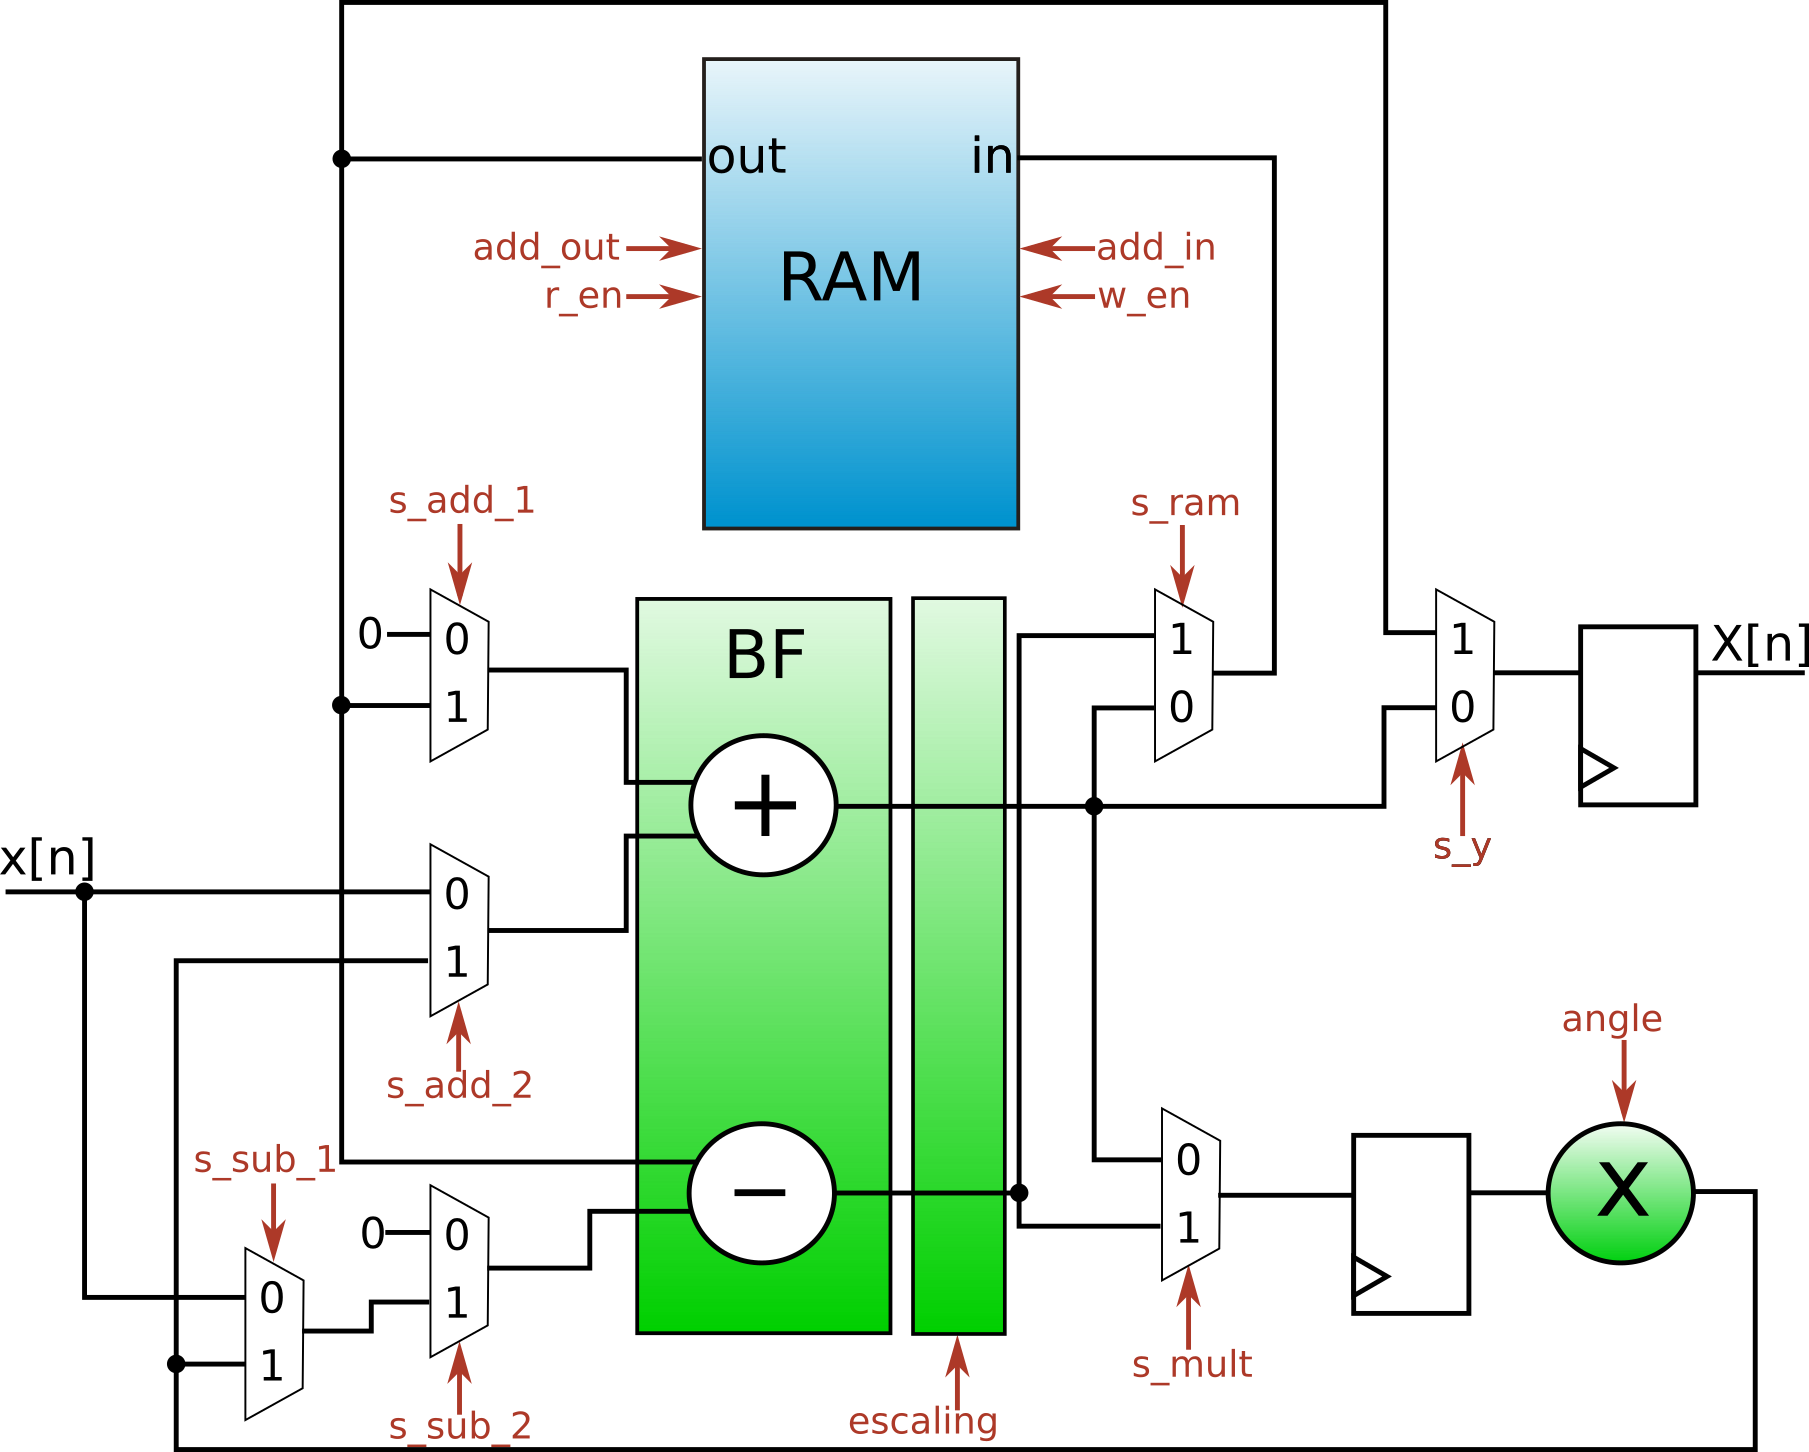
\includegraphics[width=13cm]{./figures/datapathMem.png}
				        \caption{Radix-2 implementation diagram}
				        \label{fig:datapathmem}
				\end{figure}
			\end{column}
			\begin{column}{.45\textwidth}
				\begin{figure}[htb!]
				        \centering
				        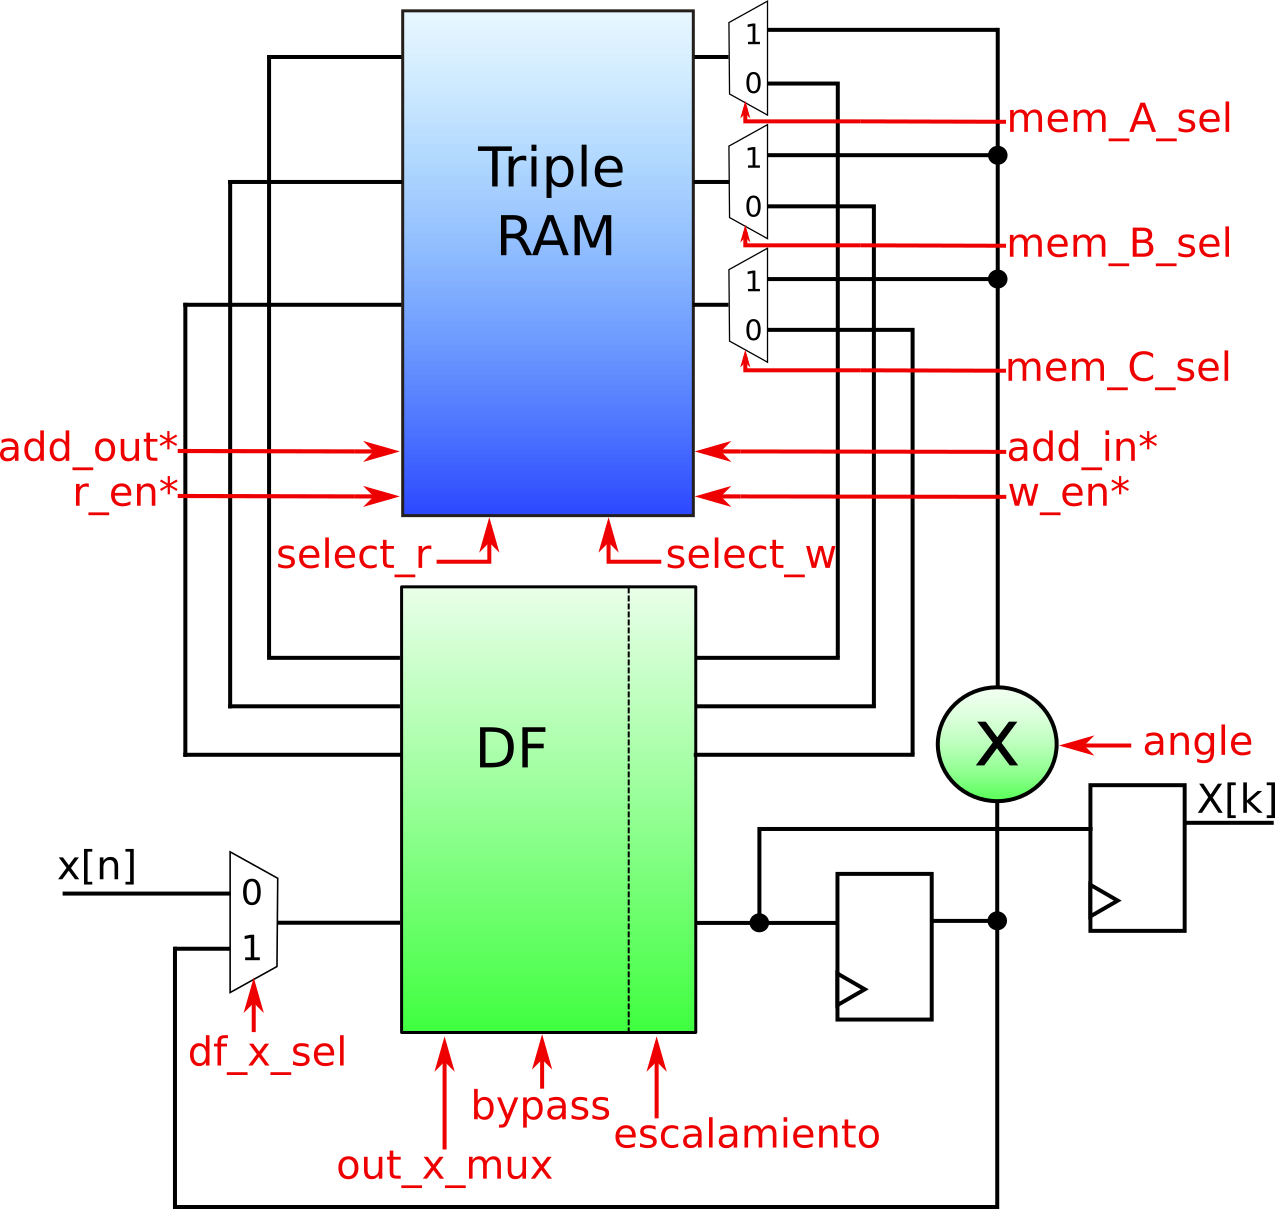
\includegraphics[width=12cm]{./figures/r4control.png}
				        \caption{Radix-4 implementation diagram}
				        \label{fig:datapathR4control}
				\end{figure}
			\end{column}
	      
	    \end{block}
% END MESA algorithm
%%%%%%%%%%%%%%%%%%%%%%%%%%%%%%%%%%%%%%%%%%%%%%%%%%%%%%%%%%%%%%%%%%%%%%%%%%%%%%%

      }
      \end{minipage}
   \end{beamercolorbox}
\end{column}
% -----------------------------------------------------------------------------
% end the column
% END first column
%%%%%%%%%%%%%%%%%%%%%%%%%%%%%%%%%%%%%%%%%%%%%%%%%%%%%%%%%%%%%%%%%%%%%%%%%%%%%%%
%%%%%%%%%%%%%%%%%%%%%%%%%%%%%%%%%%%%%%%%%%%%%%%%%%%%%%%%%%%%%%%%%%%%%%%%%%%%%%%




%%%%%%%%%%%%%%%%%%%%%%%%%%%%%%%%%%%%%%%%%%%%%%%%%%%%%%%%%%%%%%%%%%%%%%%%%%%%%%%
%%%%%%%%%%%%%%%%%%%%%%%%%%%%%%%%%%%%%%%%%%%%%%%%%%%%%%%%%%%%%%%%%%%%%%%%%%%%%%%
% BEGIN second column
% -----------------------------------------------------------------------------
% Set up a column
\begin{column}{.5\textwidth}
   \begin{beamercolorbox}[center,wd=\textwidth]{postercolumn}
      \begin{minipage}[T]{.99\textwidth}
      \parbox[t][105cm]{\textwidth}{
%%%%%%%%%%%%%%%%%%%%%%%%%%%%%%%%%%%%%%%%%%%%%%%%%%%%%%%%%%%%%%%%%%%%%%%%%%%%%%%
% BEGIN MESA algorithm continuation

		\begin{block}{Characterization}
		\justify
			Beside of the individual tests for every composing unit, a set of tests is performed over the entire architectures in order to verify and validate the design.
			For a complete description of tests and results, refer to the article related to this poster.
			
			\begin{column}{.37\textwidth}
				In order to measure the architecture error, the 64 bits floating point Matlab FFT is taken as a benchmark.

				Two metrics are used for error measuring, maximum relative error, $E_\infty$, and root mean square error, $E_2$:
				%
				\begin{equation}
				E_\infty = \max\left(\frac{ X_o[n] - X_{dut}[n]}{X_o[n]}\right)
				\label{eq:norma1}
				\end{equation}
				%
				\begin{equation}
				E_2 = \left\Vert\frac{X_o[n] - X_{dut}[n]}{X_o[n]}\right\Vert_2
				\label{eq:norma2}
				\end{equation}
				where $X_o[n]$ is the Matlab FFT output and $X_{dut}[n]$ is the design under test output.
				
			\end{column}
			\vrule
			\begin{column}{.52\textwidth}
				\begin{table}[htb!]
				\caption{$E_\infty$ for 1024 simulations, random inputs}
				\begin{tabular}{l c c}
				 & \textbf{1024 points} & \textbf{4096 points}\\ \hline 
				\textbf{R-2, Cordic} & $0.006$ & $0.008 $\\
				\textbf{R-2, Mult.} & $0.003$ & $0.108$\\
				\textbf{R-4, Cordic} & $0.003$ & $0.007$\\
				\textbf{R-4, Mult.} & $0.002$ & $0.105$\\\hline
				\end{tabular}
				\label{table:errorInf}
				\end{table}
				%
				\begin{table}[htb!]
				\caption{$E_2$ for 1024 simulations, random inputs}
				\begin{tabular}{l c c}
				 & \textbf{1024 points} & \textbf{4096 points}\\ \hline 
				\textbf{R-2, Cordic} & $0.007$  & $0.053$\\
				\textbf{R-2, Mult.} & $0.004$ & $0.131$\\
				\textbf{R-4, Cordic} & $0.002$ & $0.027$\\
				\textbf{R-4, Mult.} & $0.003$ & $0.126$\\\hline 
				\end{tabular}
				\label{table:error2}
				\end{table}
			\end{column}
			
			\begin{column}{.32\textwidth}
			The main requirement for the design is the low space/resource occupation. $16$ bits iterative radix-2 and radix-4 architectures are 
			synthesized and compared with a $16$ bits radix-2 sdf and Xilinx's LogiCORE FFT v7.1.
				
			\end{column}
			\vrule
			\begin{column}{.57\textwidth}
				\begin{table}[htb!]
				\caption{Resource occupation for $1024$ points}
				\begin{tabular}{l c c c c}
				 & \textbf{Slices} & \textbf{LUTs} & \textbf{Reg} & \textbf{LUTRAM}\\ \hline 
				\textbf{r2, cordic} & $855$ & $2712$ & $164$ & $1024$\\
				\textbf{r2, mult} & $659$ & $1884$ & $163$ & $1024$\\
				\textbf{r4, cordic} & $916$ & $2862$ & $165$ & $1152$\\
				\textbf{r4, mult} & $824$ & $2241$ & $260$ & $1152$\\
				\textbf{r2} & $3369$ & $11386$ & $1425$ & $1056$\\
				\textbf{Xilinx FFT} & $1050$ & $2541$ & $3684$ & $ $\\ \hline
				\end{tabular}
				\label{table:res1024}
				\end{table}
				%
% 				\begin{table}[htb!]
% 				\caption{Resource occupation for $4096$ points}
% 				\begin{tabular}{l c c c c}
% 				 & \textbf{Slices} & \textbf{LUTs} & \textbf{Reg} & \textbf{LUTRAM}\\ \hline 
% 				\textbf{r2-iter, cordic} & $1977$ & $6355$ & $174$ & $4096$\\
% 				\textbf{r2-iter, mult} & $1825$ & $5857$ & $174$ & $4096$\\
% 				\textbf{r4-iter, cordic} & $1941$ & $6490$ & $282$ & $4224$\\
% 				\textbf{r4-iter, mult} & $1886$ & $6202$ & $279$ & $4224$\\
% 				\textbf{r2-sdf} & $4705$ & $17405$ & $4678$ & $4128$\\
% 				\textbf{Xilinx FFT v7} & $1288$ & $3168$ & $4600$ & $ $\\ \hline
% 				\end{tabular}
% 				\label{table:res4096}
% 				\end{table}
			\end{column}
			
			\begin{column}{.39\textwidth}
			In order to meassure the ISDB-T utilization potential, the core is compared with an implementation made specifically for this use.\\
			
			The proposed core has lower resource ocupation and provides scaling options.			
			\end{column}
			\vrule
			\begin{column}{.50\textwidth}
				\begin{table}[htb!]
				\caption{Comparison with ISDB-T oriented FFT IP Core}
				\begin{tabular}{l c c }
				 & \textbf{Iter. r-2} & \textbf{Ref. IP core}\\ \hline 
				\textbf{FF} & $533$ & $1334$\\
				\textbf{LUT} & $3046$ & $4133$\\
				\textbf{BRAM} & $62$ & $62$\\
				\textbf{MUL} & $ $ & $48$\\ 
				\textbf{MHz} & $107$ & $61$\\ \hline
				\end{tabular}
				\label{table:iberchipcomp}
				\end{table}
			\end{column}
			
		\end{block}
		
		
		% END MESA algorithm continuation
%%%%%%%%%%%%%%%%%%%%%%%%%%%%%%%%%%%%%%%%%%%%%%%%%%%%%%%%%%%%%%%%%%%%%%%%%%%%%%%


%%%%%%%%%%%%%%%%%%%%%%%%%%%%%%%%%%%%%%%%%%%%%%%%%%%%%%%%%%%%%%%%%%%%%%%%%%%%%%%
% BEGIN Conclusion and future work
        \begin{block}{Conclusion and future work}
          \justify
          This paper presented two iterative radix-r FFT computing cores, designed for OFDM
			communication systems, as are detailed below:
			%
			\begin{itemize}
			  \item Radix-2 iterative architecture.
			  \item Radix-4 iterative architecture.
			  \item Cordic algorithm for twiddle factors multiplications, for radix-2 and radix-4.
			  \item Efficient complex multiplier for twiddle factors multiplications, for radix-2 and radix-4, as an alternative to 
			  cordic algorithm.
			  \item Run time, stage selectible rounding/clipping module. 
			\end{itemize} 
			%
			The cores fulfill the implementation requirements in terms of number of samples, run time configuration and scaling options.
			
			The low space/resource requirement is achieved, which made them suitable for
			integration in large systems without impacting in the resource distribution, in case of FPGA implementation, or space in case of
			ASIC implementation. 
			For future work, it can be considered to add a dithering system, in order to reduce the noise generated by the architectures, and 
			to implement a pipelined cordic without modifying the global architecture timing, in order to improve the throughput. 
        \end{block}
% END Conclusion and future work
%%%%%%%%%%%%%%%%%%%%%%%%%%%%%%%%%%%%%%%%%%%%%%%%%%%%%%%%%%%%%%%%%%%%%%%%%%%%%%%

      }
      \end{minipage}
   \end{beamercolorbox}
\end{column}
% ---------------------------------------------------------%
% end the column
% END second column
%%%%%%%%%%%%%%%%%%%%%%%%%%%%%%%%%%%%%%%%%%%%%%%%%%%%%%%%%%%%%%%%%%%%%%%%%%%%%%%
%%%%%%%%%%%%%%%%%%%%%%%%%%%%%%%%%%%%%%%%%%%%%%%%%%%%%%%%%%%%%%%%%%%%%%%%%%%%%%%




\end{columns}
%%%%%%%%%%%%%%%%%%%%%%%%%%%%%%%%%%%%%%%%%%%%%%%%%%%%%%%%%%%%%%%%%%%%%%%%%%%%%%%
\vskip1ex
\end{frame}
\end{document}
%%%%%%%%%%%%%%%%%%%%%%%%%%%%%%%%%%%%%%%%%%%%%%%%%%%%%%%%%%%%%%%%%%%%%%%%%%%%%%%
